\section{Results}
\label{sec:results}

\subsection{Color recovery pipelines}

% Generated by scripts/make_tables.py. Do not edit.
\begin{table}[t]
\centering
\small
\caption{Color recovery pipelines, all fed the same module samples: bit error rate before
Reed-Solomon correction and symbol decode rate, in percent, over the photographs localized
at the right version (4600 on CUHK-CQRC, 2456 on qrism). Centroid: nearest calibration
centroid; interf.\ canc.: interference cancellation; ours: RDA with leak inversion. Ours
decodes more symbols than every baseline, with exact McNemar $p<10^{-21}$.}
\label{tab:baselines}
\setlength{\tabcolsep}{4pt}
\begin{tabular}{@{}lrrrr@{}}
\toprule
 & \multicolumn{2}{c}{CUHK-CQRC} & \multicolumn{2}{c}{qrism} \\
\cmidrule(lr){2-3}\cmidrule(l){4-5}
Pipeline & BER & Symbol & BER & Symbol \\
\midrule
Centroid, RGB & 5.90 & 19.9 & 7.18 & 16.4 \\
Centroid, optical density & 7.31 & 12.4 & 10.30 & 5.8 \\
Centroid, black/white stretch & 5.96 & 20.0 & 7.19 & 16.5 \\
\midrule
Interf. canc., density & 6.91 & 14.3 & 7.92 & 18.5 \\
Interf. canc., absorptance & 6.25 & 14.6 & -- & -- \\
Interf. canc., local thr. & 6.75 & 18.0 & -- & -- \\
Local threshold & 16.61 & 0.0 & -- & -- \\
JAB Code classifier & -- & -- & 8.89 & 13.2 \\
\midrule
LDA & 5.54 & 32.2 & 6.23 & 22.3 \\
QDA & 6.10 & 21.2 & 9.21 & 12.9 \\
RDA ($\lambda=0.5$) & 5.29 & 35.4 & 5.90 & 24.3 \\
\midrule
Ours, $\beta$ fit per image & 5.00 & 39.3 & -- & -- \\
\textbf{Ours, $\beta=0.06$} & \textbf{4.61} & \textbf{42.9} & \textbf{4.85} & \textbf{33.9} \\
\bottomrule
\end{tabular}
\end{table}


Table~\ref{tab:baselines} compares color recovery pipelines on both datasets. Nearest
centroid in raw RGB decodes \HiqCodeEuclid\% of symbols on CUHK-CQRC and \QrCodeEuclid\% on
qrism, and per-colorant interference cancellation~\cite{blasinski2013pccc}
\HiqCodePerColorant\% and \QrCodePerColorant\%. JAB Code's classifier decodes \QrCodeJab\%
on qrism. Keeping the same centroids but measuring distance with the RDA metric raises the
rate to \HiqCodeRda\% and \QrCodeRda\%, and adding leak inversion at $\beta=0.06$ raises it to
\HiqCodeChosen\% (95\% CI \HiqCodeChosenLo--\HiqCodeChosenHi) and \QrCodeChosen\%
(\QrCodeChosenLo--\QrCodeChosenHi). Every baseline decodes fewer symbols than our method on
both datasets; the closest has exact McNemar $p\BaselineWorstP$. Leak inversion alone decodes
\HiqDeblurGainOnly{} CUHK-CQRC photographs that RDA misses and loses \HiqDeblurLossOnly{}
($p\HiqDeblurP$); on qrism the counts are \QrDeblurGainOnly{} and \QrDeblurLossOnly{}
($p\QrDeblurP$).

Module accuracy understates these differences. Nearest centroid and our method differ by
three points in module accuracy (\HiqDataEuclid\% against \HiqDataChosen\%) but by more than
a factor of two in symbols decoded, because a symbol fails as soon as one Reed-Solomon
block in one layer holds more errors than it can correct. We therefore rank pipelines and
choose parameters by symbol decode rate.

Choosing $\beta$ per photograph does worse than the fixed value: minimizing the spread of
the corrected grid around its palette gives \HiqCodeFit\%, and an optical estimate of
blur measured on the finder edges gives \HiqCodeOptical\%.

\subsection{Leak fraction}

\begin{figure}[t]
\centering
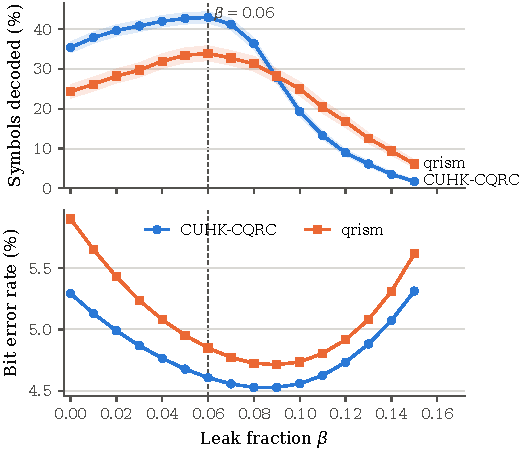
\includegraphics[width=\columnwidth]{generated/fig_beta.pdf}
\caption{Leak fraction $\beta$ against symbol decode rate with its 95\% Wilson band (top)
and pre-correction bit error rate (bottom), RDA shrink $\lambda=0.5$. $\beta=0$ is RDA
without leak inversion. Each dataset's photographs are those localized at the right
version.}
\label{fig:beta}
\end{figure}

Fig.~\ref{fig:beta} sweeps $\beta$ from 0 to 0.15. On each dataset separately the decode
rate peaks at $\beta=0.06$: \HiqCodeChosen\% on CUHK-CQRC against \HiqCodeNoDeblur\%
without leak inversion, and \QrCodeChosen\% on the qrism dataset against
\QrCodeNoDeblur\%. Because both datasets select the same value, choosing $\beta$ on one
and testing on the other costs nothing. The optimum is narrow but not sharp: $\beta=0.05$
cannot be told apart from 0.06 ($p\HiqPFive$ and $p\QrPFive$), while 0.04 ($p\HiqPFour$,
$p\QrPFour$) and 0.07 ($p\HiqPSeven$, $p\QrPSeven$) are worse on both datasets. Past 0.08
the noise gain dominates and decoding collapses, to \HiqCodeTwelve\% and \QrCodeTwelve\%
at $\beta=0.12$.

The bit error rate does not peak where decoding does. At $\beta=0.06$ it falls from
\HiqBerNoDeblur\% to \HiqBerChosen\% on CUHK-CQRC and from \QrBerNoDeblur\% to
\QrBerChosen\% on qrism, but it keeps falling, to $\beta=\HiqBerMinBeta$ on CUHK-CQRC and
\QrBerMinBeta{} on qrism. Our reading is that the photographs that can be decoded at all
want less correction than those that cannot. On
the qrism dataset the bit error rate of 20\,px symbols is lowest at
$\beta=\QrBerMinBetaPxTwenty$, next to their decode optimum, while 12\,px and 8\,px
symbols, which rarely decode, are best served by $\beta=\QrBerMinBetaPxTwelve$ and
\QrBerMinBetaPxEight. Those symbols pull the pooled bit error rate toward larger $\beta$
without adding decoded symbols. The per-photograph optical estimate shows the same split:
it has the lowest bit error rate of any setting on both datasets, yet on CUHK-CQRC it
decodes fewer symbols than the fixed value (\HiqCodeOptical\% against \HiqCodeChosen\%,
$p\HiqPOptical$); on qrism the two tie (\QrCodeOptical\% against \QrCodeChosen\%,
$p\QrPOptical$).

Blue is the weakest channel on both datasets. At $\beta=0.06$ its bit error rate is
\HiqBerChosenB\% on CUHK-CQRC against \HiqBerChosenR\% and \HiqBerChosenG\% for red and
green, and \QrBerChosenB\% on qrism against \QrBerChosenR\% and \QrBerChosenG\%. HiQ
reports the same for its third layer~\cite{yang2018hiq}. Since a qrism symbol decodes only
when all three channels do, the blue channel bounds its decode rate.

\subsection{Covariance shrink}

% Generated by scripts/make_tables.py. Do not edit.
\begin{table}[t]
\centering
\small
\caption{Symbol decode rate (\%) against the RDA shrink $\lambda$, without leak
inversion ($\beta=0$) and with it ($\beta=0.06$).}
\label{tab:shrink}
\begin{tabular}{@{}lrrrr@{}}
\toprule
 & \multicolumn{2}{c}{CUHK-CQRC} & \multicolumn{2}{c}{qrism} \\
\cmidrule(lr){2-3}\cmidrule(l){4-5}
$\lambda$ & $\beta=0$ & $0.06$ & $\beta=0$ & $0.06$ \\
\midrule
0.0 (QDA) & 21.2 & 28.6 & 12.9 & 17.8 \\
0.2 & 33.6 & 39.5 & 21.5 & 31.6 \\
0.4 & 35.5 & 42.5 & 23.5 & 33.3 \\
0.5 (used) & \textbf{35.4} & \textbf{42.9} & \textbf{24.3} & \textbf{33.9} \\
0.6 & 34.9 & 43.1 & 24.6 & 33.9 \\
0.8 & 33.7 & 42.8 & 24.3 & 33.0 \\
1.0 (LDA) & 32.2 & 41.9 & 22.3 & 30.0 \\
\bottomrule
\end{tabular}
\end{table}


Table~\ref{tab:shrink} crosses the RDA shrink $\lambda$ with $\beta$. Decode rates are flat
for $\lambda$ between 0.4 and 0.7 and fall at both ends. With leak inversion, QDA decodes
\HiqCodeQda\% on CUHK-CQRC ($p\HiqPQda$ against $\lambda=0.5$) and \QrCodeQda\% on qrism
($p\QrPQda$): per-class covariances estimated from few samples (17 for black on
CUHK-CQRC), then amplified by the correction, generalize poorly. LDA loses less, \HiqCodeLda\% ($p\HiqPLda$)
and \QrCodeLda\% ($p\QrPLda$). The best cell of the full grid is \HiqGridBest{} on CUHK-CQRC
(\HiqGridBestCode\%, $p\HiqGridBestP$ against $\lambda=0.5$) and \QrGridBest{} on qrism. For
every $\lambda \geq 0.3$ the best $\beta$ is \GridBestBetaRange, so the two parameters can
be set independently.

\subsection{Module size and capture condition}

% Generated by scripts/make_tables.py. Do not edit.
\begin{table}[t]
\centering
\small
\caption{qrism dataset: symbol decode rate (\%) by module size and capture condition,
without leak inversion, at $\beta=0.06$, and at the best fixed $\beta$ for that
group. $n$ is localized photos.}
\label{tab:breakdown}
\begin{tabular}{@{}lrrrrr@{}}
\toprule
Group & $n$ & $\beta=0$ & $0.06$ & best $\beta$ & at best \\
\midrule
0.34 mm & 263 & 52.1 & 46.0 & 0.03 & 54.8 \\
0.5 mm & 1061 & 9.3 & 18.5 & 0.08 & 19.8 \\
0.84 mm & 1136 & 43.8 & 56.0 & 0.06 & 56.0 \\
\midrule
regular & 1024 & 27.8 & 39.8 & 0.05 & 40.5 \\
daylight & 271 & 46.1 & 41.3 & 0.01 & 49.1 \\
flashlight & 458 & 14.0 & 28.4 & 0.10 & 31.0 \\
monitor & 75 & 90.7 & 89.3 & 0.01 & 92.0 \\
close & 28 & 82.1 & 85.7 & 0.02 & 85.7 \\
wb-cool & 23 & 30.4 & 47.8 & 0.10 & 65.2 \\
wb-neutral & 145 & 11.7 & 35.9 & 0.10 & 55.2 \\
wb-warm & 173 & 4.0 & 16.2 & 0.06 & 16.2 \\
\bottomrule
\end{tabular}
\end{table}


Table~\ref{tab:breakdown} breaks the qrism results down. The best $\beta$ grows as modules
shrink: \QrBestBetaPxTwenty{} at 20\,px, \QrBestBetaPxTwelve{} at 12\,px and
\QrBestBetaPxEight{} at 8\,px. This is what a blur of fixed width in pixels predicts, since
it covers a larger fraction of a smaller module. At 8\,px almost nothing decodes, at most
\QrBestCodePxEight\%. Capture conditions move the optimum as well: daylight photographs do
best at $\beta=\QrBestBetaDaylight$ (\QrBestCodeDaylight\% against \QrCodeChosenDaylight\%
at 0.06), while the neutral white-balance condition does best at \QrBestBetaWbNeutral{} and
the flash condition at \QrBestBetaFlashlight. These per-group optima are chosen on the photographs they are
scored on, so they overstate what a per-group $\beta$ would gain; they show that a single
$\beta$ is a compromise across conditions.

\subsection{Comparison with the HiQ decoder}
\label{sec:hiq}

% Generated by scripts/make_tables.py. Do not edit.
\begin{table}[t]
\centering
\small
\caption{End-to-end decoders on HiQ's test split of CUHK-CQRC, paired by photo. Each decoder uses its own
localization and sampling. CMI, corrected: all five CMI weights, with the neighbors HiQ's
sampler gathers (two of four on most modules). Disc.: photos only ours decoded / only HiQ
decoded; every difference has exact McNemar $p<10^{-127}$.}
\label{tab:paired}
\setlength{\tabcolsep}{4pt}
\begin{tabular}{@{}lrcr@{}}
\toprule
Decoder & Symbol \% & 95\% CI & Disc. \\
\midrule
\multicolumn{4}{@{}l}{\emph{Localized by both ($n=3404$)}} \\
Ours, $\beta=0.06$ & 50.1 & [48.4, 51.7] & \\
HiQ QDA & 26.0 & [24.6, 27.5] & 926/108 \\
HiQ QDA + CMI, corrected & 29.5 & [28.0, 31.0] & 824/123 \\
HiQ layered SVM & 25.5 & [24.1, 27.0] & 931/95 \\
\midrule
\multicolumn{4}{@{}l}{\emph{All photos ($n=5381$)}} \\
Ours, $\beta=0.06$ & 35.3 & [34.0, 36.5] & \\
HiQ QDA & 17.2 & [16.2, 18.3] & 1119/149 \\
HiQ QDA + CMI, corrected & 19.5 & [18.4, 20.5] & 1017/167 \\
HiQ layered SVM & 16.7 & [15.7, 17.7] & 1124/126 \\
\bottomrule
\end{tabular}
\end{table}


This comparison uses only HiQ's test split, so no photograph HiQ's models were trained on is
scored. Of its \PairTest{} photographs the HiQ decoder localizes \PairHiqLocalized{} and ours
\PairOursLocalized; \PairBoth{} are localized by both, \PairCommon{} of them at the same
version. Table~\ref{tab:paired} compares the decoders on these photographs and
on all photographs, counting a photograph that a decoder does not localize as a failure.
On the common set our decoder reads \PairCommonOurs\% of symbols against \PairCommonHiq\%
for HiQ's best configuration, QDA with the corrected CMI. It leads in all
\PairVersionsTotal{} symbol versions and all \PairFoldersTotal{} capture folders. Without
leak inversion it reads \PairCommonOursNoDeblur\%, still ahead of HiQ.

The HiQ classifiers were also timed on the same machine, over the same span as ours
(Section~\ref{sec:method}): \HiqTimeLsvmNs\,ns per module for the layered SVM,
\HiqTimeQdaNs\,ns for QDA and \HiqTimeQdaCmiNs\,ns for QDA with the corrected CMI, against
\TimeChosenNs\,ns for ours. These figures do not isolate the algorithms. HiQ runs as
JIT-compiled Java and ours as Rust, which favors ours; HiQ fits nothing per photograph while
our time includes the fit, which favors HiQ. They do show that the costs are of the same order:
ours falls between HiQ's layered SVM and its QDA without any training, and the layered SVM,
the only faster one, decodes \PairCommonLsvm\% of the common set.

One qualification applies. Each decoder uses its own localization and module sampling, so
the gap combines color recovery and sampling; a comparison of the classifiers alone needs
HiQ's classifier run on our samples. \todo{run HiQ's QDA and corrected CMI on the library's
samples, or state the claim as end-to-end only}
